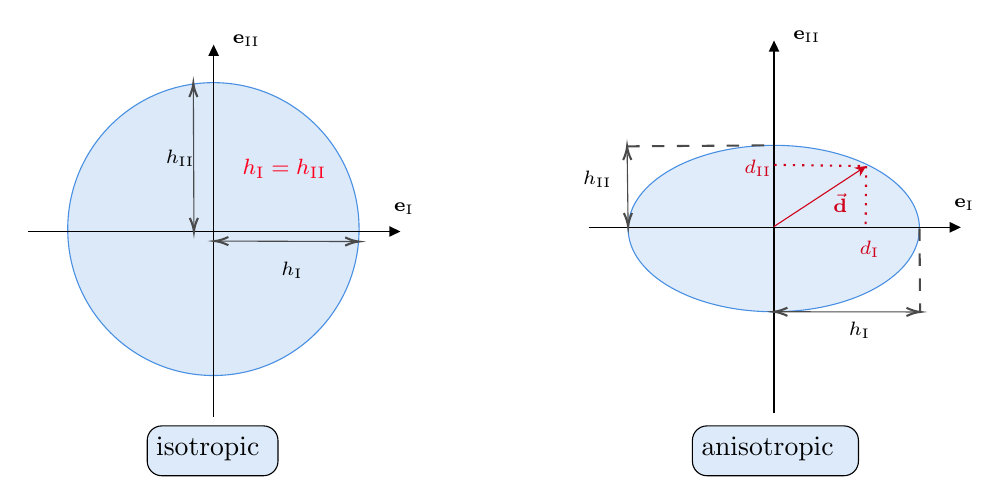
\begin{tikzpicture}[x=0.75pt,y=0.75pt,yscale=-1,xscale=1]
%uncomment if require: \path (0,365); %set diagram left start at 0, and has height of 365

%Shape: Ellipse [id:dp47149657789461774] 
\draw  [color={rgb, 255:red, 74; green, 144; blue, 226 }  ,draw opacity=1 ][fill={rgb, 255:red, 74; green, 144; blue, 226 }  ,fill opacity=0.2 ] (80.03,160.17) .. controls (80.03,121.2) and (111.45,89.62) .. (150.21,89.62) .. controls (188.98,89.62) and (220.4,121.2) .. (220.4,160.17) .. controls (220.4,199.13) and (188.98,230.72) .. (150.21,230.72) .. controls (111.45,230.72) and (80.03,199.13) .. (80.03,160.17) -- cycle ;
%Straight Lines [id:da9023088519674093] 
\draw    (61,161.33) -- (237.33,161.33) ;
\draw [shift={(240.33,161.33)}, rotate = 180] [fill={rgb, 255:red, 0; green, 0; blue, 0 }  ][line width=0.08]  [draw opacity=0] (5.36,-2.57) -- (0,0) -- (5.36,2.57) -- cycle    ;
%Straight Lines [id:da8803342561855532] 
\draw    (150.33,250.67) -- (150.33,74.33) ;
\draw [shift={(150.33,71.33)}, rotate = 90] [fill={rgb, 255:red, 0; green, 0; blue, 0 }  ][line width=0.08]  [draw opacity=0] (5.36,-2.57) -- (0,0) -- (5.36,2.57) -- cycle    ;
%Straight Lines [id:da970968031905884] 
\draw [color={rgb, 255:red, 74; green, 74; blue, 74 }  ,draw opacity=1 ]   (140.83,159.36) -- (140.56,91.95) ;
\draw [shift={(140.55,89.95)}, rotate = 89.77] [color={rgb, 255:red, 74; green, 74; blue, 74 }  ,draw opacity=1 ][line width=0.75]    (6.56,-1.97) .. controls (4.17,-0.84) and (1.99,-0.18) .. (0,0) .. controls (1.99,0.18) and (4.17,0.84) .. (6.56,1.97)   ;
\draw [shift={(140.83,161.36)}, rotate = 269.77] [color={rgb, 255:red, 74; green, 74; blue, 74 }  ,draw opacity=1 ][line width=0.75]    (6.56,-1.97) .. controls (4.17,-0.84) and (1.99,-0.18) .. (0,0) .. controls (1.99,0.18) and (4.17,0.84) .. (6.56,1.97)   ;
%Straight Lines [id:da687532719461613] 
\draw [color={rgb, 255:red, 74; green, 74; blue, 74 }  ,draw opacity=1 ]   (152.86,165.94) -- (218.27,166.17) ;
\draw [shift={(220.27,166.18)}, rotate = 180.2] [color={rgb, 255:red, 74; green, 74; blue, 74 }  ,draw opacity=1 ][line width=0.75]    (6.56,-1.97) .. controls (4.17,-0.84) and (1.99,-0.18) .. (0,0) .. controls (1.99,0.18) and (4.17,0.84) .. (6.56,1.97)   ;
\draw [shift={(150.86,165.94)}, rotate = 0.2] [color={rgb, 255:red, 74; green, 74; blue, 74 }  ,draw opacity=1 ][line width=0.75]    (6.56,-1.97) .. controls (4.17,-0.84) and (1.99,-0.18) .. (0,0) .. controls (1.99,0.18) and (4.17,0.84) .. (6.56,1.97)   ;
%Shape: Ellipse [id:dp2890703530536485] 
\draw  [color={rgb, 255:red, 74; green, 144; blue, 226 }  ,draw opacity=1 ][fill={rgb, 255:red, 74; green, 144; blue, 226 }  ,fill opacity=0.17 ] (350.03,159.91) .. controls (350.03,137.76) and (381.45,119.81) .. (420.21,119.81) .. controls (458.98,119.81) and (490.4,137.76) .. (490.4,159.91) .. controls (490.4,182.05) and (458.98,200) .. (420.21,200) .. controls (381.45,200) and (350.03,182.05) .. (350.03,159.91) -- cycle ;
%Straight Lines [id:da7491324989595073] 
\draw    (331,159.33) -- (507.33,159.33) ;
\draw [shift={(510.33,159.33)}, rotate = 180] [fill={rgb, 255:red, 0; green, 0; blue, 0 }  ][line width=0.08]  [draw opacity=0] (5.36,-2.57) -- (0,0) -- (5.36,2.57) -- cycle    ;
%Straight Lines [id:da5761256453181017] 
\draw    (420.33,248.67) -- (420.33,72.33) ;
\draw [shift={(420.33,69.33)}, rotate = 90] [fill={rgb, 255:red, 0; green, 0; blue, 0 }  ][line width=0.08]  [draw opacity=0] (5.36,-2.57) -- (0,0) -- (5.36,2.57) -- cycle    ;
%Straight Lines [id:da7041621788435982] 
\draw [color={rgb, 255:red, 74; green, 74; blue, 74 }  ,draw opacity=1 ]   (350,157) -- (349.55,122.31) ;
\draw [shift={(349.53,120.31)}, rotate = 89.26] [color={rgb, 255:red, 74; green, 74; blue, 74 }  ,draw opacity=1 ][line width=0.75]    (6.56,-1.97) .. controls (4.17,-0.84) and (1.99,-0.18) .. (0,0) .. controls (1.99,0.18) and (4.17,0.84) .. (6.56,1.97)   ;
\draw [shift={(350.03,159)}, rotate = 269.26] [color={rgb, 255:red, 74; green, 74; blue, 74 }  ,draw opacity=1 ][line width=0.75]    (6.56,-1.97) .. controls (4.17,-0.84) and (1.99,-0.18) .. (0,0) .. controls (1.99,0.18) and (4.17,0.84) .. (6.56,1.97)   ;
%Straight Lines [id:da33821473867960394] 
\draw [color={rgb, 255:red, 74; green, 74; blue, 74 }  ,draw opacity=1 ]   (422.21,200) -- (488.71,200.1) ;
\draw [shift={(490.71,200.1)}, rotate = 180.08] [color={rgb, 255:red, 74; green, 74; blue, 74 }  ,draw opacity=1 ][line width=0.75]    (6.56,-1.97) .. controls (4.17,-0.84) and (1.99,-0.18) .. (0,0) .. controls (1.99,0.18) and (4.17,0.84) .. (6.56,1.97)   ;
\draw [shift={(420.21,200)}, rotate = 0.08] [color={rgb, 255:red, 74; green, 74; blue, 74 }  ,draw opacity=1 ][line width=0.75]    (6.56,-1.97) .. controls (4.17,-0.84) and (1.99,-0.18) .. (0,0) .. controls (1.99,0.18) and (4.17,0.84) .. (6.56,1.97)   ;
%Straight Lines [id:da09564868493828071] 
\draw [color={rgb, 255:red, 208; green, 2; blue, 27 }  ,draw opacity=1 ]   (420.21,159) -- (462.21,131.46) ;
\draw [shift={(464.71,129.81)}, rotate = 146.74] [fill={rgb, 255:red, 208; green, 2; blue, 27 }  ,fill opacity=1 ][line width=0.08]  [draw opacity=0] (5.36,-2.57) -- (0,0) -- (5.36,2.57) -- (3.56,0) -- cycle    ;
%Straight Lines [id:da7191734000127111] 
\draw [color={rgb, 255:red, 74; green, 74; blue, 74 }  ,draw opacity=1 ][line width=0.75]  [dash pattern={on 4.5pt off 4.5pt}]  (349.53,120.31) -- (420.21,119.81) ;
%Straight Lines [id:da23417744915968897] 
\draw [color={rgb, 255:red, 74; green, 74; blue, 74 }  ,draw opacity=1 ][line width=0.75]  [dash pattern={on 4.5pt off 4.5pt}]  (490.4,159.91) -- (490.71,200.1) ;
%Straight Lines [id:da9599209932665848] 
\draw [color={rgb, 255:red, 208; green, 2; blue, 27 }  ,draw opacity=1 ][line width=0.75]  [dash pattern={on 0.84pt off 2.51pt}]  (420.43,129.24) -- (464.71,129.81) ;
%Straight Lines [id:da46869669446608475] 
\draw [color={rgb, 255:red, 208; green, 2; blue, 27 }  ,draw opacity=1 ][line width=0.75]  [dash pattern={on 0.84pt off 2.51pt}]  (464.71,129.81) -- (464.43,160.1) ;

% Text Node
\draw (126,120.73) node [anchor=north west][inner sep=0.75pt]  [font=\scriptsize]  {$h_{\mathrm{II}}$};
% Text Node
\draw (181.67,174.73) node [anchor=north west][inner sep=0.75pt]  [font=\scriptsize]  {$h_{\mathrm{I}}$};
% Text Node
\draw (158.33,65.4) node [anchor=north west][inner sep=0.75pt]  [font=\scriptsize]  {$\mathbf{e}_{\mathrm{II}}$};
% Text Node
\draw (236,146.4) node [anchor=north west][inner sep=0.75pt]  [font=\scriptsize]  {$\mathbf{e}_{\mathrm{I}}$};
% Text Node
\draw (163,125.4) node [anchor=north west][inner sep=0.75pt]  [font=\footnotesize,color={rgb, 255:red, 255; green, 0; blue, 31 }  ,opacity=1 ]  {$h_{\mathrm{I}} =h_{\mathrm{II}}$};
% Text Node
\draw  [fill={rgb, 255:red, 74; green, 144; blue, 226 }  ,fill opacity=0.19 ]  (118.33,262) .. controls (118.33,258.13) and (121.47,255) .. (125.33,255) -- (174.33,255) .. controls (178.2,255) and (181.33,258.13) .. (181.33,262) -- (181.33,272) .. controls (181.33,275.87) and (178.2,279) .. (174.33,279) -- (125.33,279) .. controls (121.47,279) and (118.33,275.87) .. (118.33,272) -- cycle  ;
\draw (121.33,259) node [anchor=north west][inner sep=0.75pt]   [align=left] {isotropic};
% Text Node
\draw (327.05,130.92) node [anchor=north west][inner sep=0.75pt]  [font=\scriptsize]  {$h_{\mathrm{II}}$};
% Text Node
\draw (455.1,203.59) node [anchor=north west][inner sep=0.75pt]  [font=\scriptsize]  {$h_{\mathrm{I}}$};
% Text Node
\draw (428.33,63.4) node [anchor=north west][inner sep=0.75pt]  [font=\scriptsize]  {$\mathbf{e}_{\mathrm{II}}$};
% Text Node
\draw (506,144.4) node [anchor=north west][inner sep=0.75pt]  [font=\scriptsize]  {$\mathbf{e}_{\mathrm{I}}$};
% Text Node
\draw  [fill={rgb, 255:red, 74; green, 144; blue, 226 }  ,fill opacity=0.19 ]  (381,262) .. controls (381,258.13) and (384.13,255) .. (388,255) -- (454,255) .. controls (457.87,255) and (461,258.13) .. (461,262) -- (461,272) .. controls (461,275.87) and (457.87,279) .. (454,279) -- (388,279) .. controls (384.13,279) and (381,275.87) .. (381,272) -- cycle  ;
\draw (384,259) node [anchor=north west][inner sep=0.75pt]   [align=left] {anisotropic};
% Text Node
\draw (460.24,164.78) node [anchor=north west][inner sep=0.75pt]  [font=\scriptsize,color={rgb, 255:red, 208; green, 2; blue, 27 }  ,opacity=1 ]  {$d_{\mathrm{I}}$};
% Text Node
\draw (404.76,125.78) node [anchor=north west][inner sep=0.75pt]  [font=\scriptsize,color={rgb, 255:red, 208; green, 2; blue, 27 }  ,opacity=1 ]  {$d_{\mathrm{II}}$};
% Text Node
\draw (447.71,141.64) node [anchor=north west][inner sep=0.75pt]  [font=\scriptsize,color={rgb, 255:red, 208; green, 2; blue, 27 }  ,opacity=1 ]  {$\vec{\mathbf{d}}$};


\end{tikzpicture}
